Dada toda a complexidade na formulação dos fluxos 
de processamento de dados e na regularização de variáveis de ambiente, 
torna-se de extrema relevância para a compreensão da 
construção do fluxo definitivo a apresentação das principais 
ferramentas, frameworks e bibliotecas utilizadas.

\subsubsection{VSCode}
O Visual Studio Code (VSCode) é um editor de texto desenvolvido pela Microsoft em 2015, 
baseado no framework Electron (implementado em JavaScript). 
Foi utilizado neste trabalho por conta de sua simples integração com 
diversas linguagens por meio de extensões, 
sua fácil instalação na maioria dos hardwares e sistemas operacionais com foco no uso diário e, 
por não ser propriamente uma IDE, 
apresenta menor complexidade de utilização
e configuração de ambientes de desenvolvimento. A Figura~\ref{fig:vscode} mostra a sua interface.

\begin{figure}[H]
    \centering
    \caption{Interface do Visual Studio Code}
    \label{fig:vscode}
    \includegraphics[width=0.8\textwidth]{sections/imagens/VSCode_Main_PAge.png}
    \legend{Fonte: Captura de tela feita pelos autores (2026).}
\end{figure}

\paragraph{Python}
Utilizada como linguagem base no desenvolvimento de inúmeros projetos de Inteligência Artificial, 
a linguagem Python foi escolhida neste trabalho por sua versatilidade no desenvolvimento de aplicações, 
especialmente no que tange ao desenvolvimento, 
treinamento e testes de modelos de \gls{ocr} e à análise de dados, 
provendo os insumos necessários para a validação do presente estudo.

\begin{lstlisting}[language=Python, caption={Exemplo ilustrativo de código em Python}]
import argparse
import math
import enlace
CAPTURAS_REAIS = (2460, 3705, 4209, 4184)
POC_Q90 = (3151, 3310)
TAMANHO_REFERENCIA = 4300

def tempo_no_ar_ms(payload_phy: int, sf: int, bw_hz: float, preambulo: int = PREAMBULO) -> float:
    """Tempo no ar (ms) de um pacote LoRa com `payload_phy` bytes na camada fisica."""
    t_sym = (2 ** sf) / bw_hz
    de = 1 if t_sym > 0.016 else 0         # low data rate optimize
    num = (8 * payload_phy - 4 * sf + 28
           + (16 if CRC_LIGADO else 0)
           - (0 if CABECALHO_EXPLICITO else 20))
    n_payload = 8 + max(math.ceil(num / (4 * (sf - 2 * de))) * (CODING_RATE + 4), 0)
    return (preambulo + 4.25 + n_payload) * t_sym * 1000
\end{lstlisting}
\begin{center}
    \footnotesize Fonte: Autores (2026).
\end{center}

\paragraph{TensorFlow | Keras | TFLite}
As principais ferramentas para o desenvolvimento, 
treinamento, quantização, testes e validação dos modelos de \gls{ocr} 
foram os frameworks TensorFlow e Keras, com compilação de saída em arquivos \texttt{.tflite} 
compatíveis com o módulo TFLite instalado nativamente no firmware do \gls{esp32cam}, e instalado via gerenciador de pacotes pip em computadores pessoais utilizados como servidor de rede.

O TensorFlow, lançado em 2015 pelo Google,
é uma biblioteca de código aberto focada em cálculos matemáticos complexos de matrizes, 
atividade essencial para o funcionamento de redes neurais convolucionais. 
Integrado de forma homogênea ao TensorFlow, 
o Keras é uma API de alto nível desenvolvida pelo Google (lançada em 2015) 
com o foco em simplificar o desenvolvimento de redes neurais com poucas linhas de código.

O TensorFlow Lite (TFLite), oficialmente anunciado pelo Google em 2017, é a versão do TensorFlow voltada à execução de modelos de \gls{ia} em dispositivos móveis e embarcados. Sua variante para microcontroladores, o TensorFlow Lite Micro, usada no firmware deste trabalho, executa modelos minimizados em microcontroladores de desempenho limitado. Desde 2024, o TFLite foi renomeado como LiteRT, sem grandes alterações estruturais em seu funcionamento, mantendo inclusive a extensão \textit{.tflite} nos arquivos de modelo.


\subsubsection{Arduino IDE e Arduino CLI}
O Arduino IDE, lançado em 2005, é o principal ambiente de desenvolvimento integrado para
sistemas baseados em microcontroladores e uma ferramenta indispensável no desenvolvimento
\gls{iot}. Ele integra funcionalidades que facilitam a comunicação entre o computador e os
microcontroladores, servindo também como ambiente para a comunicação serial entre os
dispositivos. A sua interface é mostrada na Figura~\ref{fig:arduinoide}.

\begin{figure}[H]
    \centering
    \caption{Interface do Arduino IDE}
    \label{fig:arduinoide}
    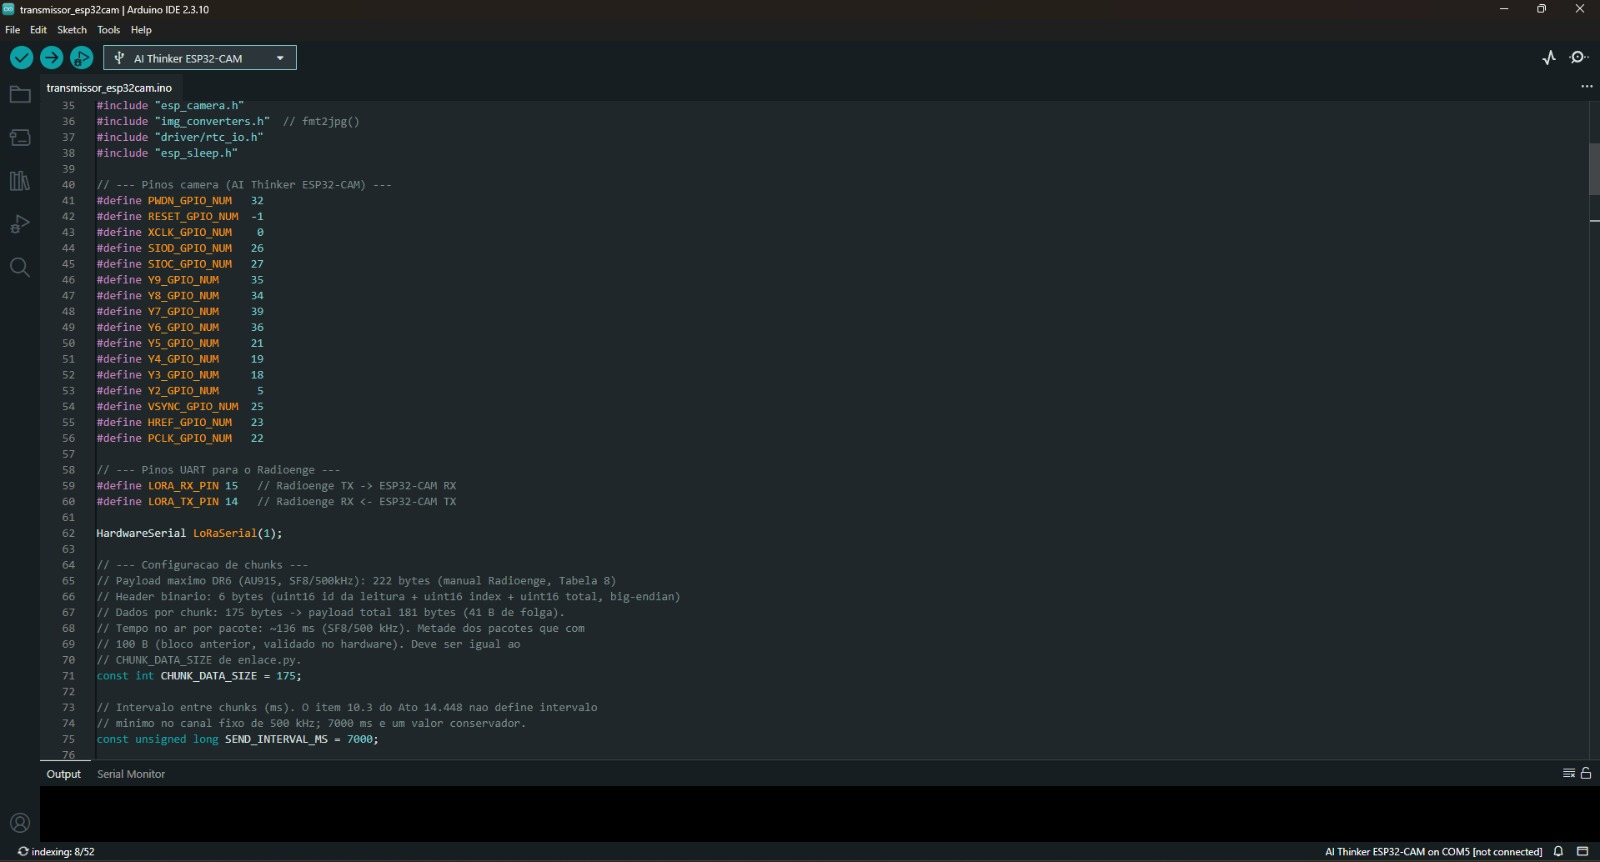
\includegraphics[width=0.8\textwidth]{sections/imagens/Arduino_IDE.jpeg}
    \legend{Fonte: Captura de tela feita pelos autores (2026).}
\end{figure}

Como complemento, a própria equipe da Arduino SA lançou, em 2018, o Arduino CLI, uma
ferramenta de linha de comando desenvolvida para agilizar compilações, testes, instalação
de bibliotecas e automação de tarefas relacionadas ao desenvolvimento de sistemas baseados
em microcontroladores.

\paragraph{C++ (.ino)}
A linguagem C++, usada nos arquivos \texttt{.ino} do core Arduino-ESP32 neste trabalho,
foi utilizada para realizar a comunicação e a orquestração de funções do 
hardware do \gls{esp32cam} e de seus módulos. 
Essa linguagem possui grande relevância no cenário de dispositivos \gls{iot} 
por proporcionar alta granularidade no controle de memória RAM 
e PSRAM alocadas às mais diversas tarefas. 

\begin{lstlisting}[language=C++, caption={Exemplo ilustrativo de código em C++ para ESP32}]
#define LORA_RX_PIN 15 // Conectado ao TX da Radioenge (Pino 3)
#define LORA_TX_PIN 14 // Conectado ao RX da Radioenge (Pino 2)

HardwareSerial LoRaSerial(1);

const unsigned long TIMEOUT_TOTAL_MS = 3000;   // Espera maxima por comando
const unsigned long SILENCIO_FIM_MS  = 400;    // Sem bytes por este tempo = resposta completa

const char *COMANDOS[] = {
  "AT+DADDR=?",
  "AT+NWKSKEY=?",
  "AT+APPSKEY=?",
  "AT+NJM=?",
};
const int N_COMANDOS = sizeof(COMANDOS) / sizeof(COMANDOS[0]);

// Envia um comando AT e devolve a resposta bruta (sem espacos nas pontas).
String consultar(const char *cmd) {
  while (LoRaSerial.available()) LoRaSerial.read(); // Descarta lixo pendente
  LoRaSerial.println(cmd);

  String resposta = "";
  unsigned long inicio = millis();
  unsigned long ultimoByte = 0;

  while (millis() - inicio < TIMEOUT_TOTAL_MS) {
    while (LoRaSerial.available()) {
      resposta += (char)LoRaSerial.read();
      ultimoByte = millis();
    }
    if (resposta.length() > 0 && millis() - ultimoByte > SILENCIO_FIM_MS) break;
    delay(5);
  }
  resposta.trim();
  return resposta;
}
\end{lstlisting}
\begin{center}
    \footnotesize Fonte: Autores (2026).
\end{center}


\subsubsection{Git e GitHub}
O GitHub, plataforma de versionamento online de códigos 
mais difundida na comunidade de desenvolvimento mundial, 
criada em 2008 e atualmente dirigida pela Microsoft, 
foi utilizado com o objetivo de armazenar repositórios
e transparecer a evolução do trabalho a todos os integrantes (Figura~\ref{fig:github}).

Integrado ao GitHub, 
outra ferramenta de suma importância na orquestração e 
gestão do versionamento é o Git. Criada por Linus Torvalds em 2005, 
essa ferramenta tem como objetivo prover insumos para o versionamento de 
código estruturado e integrar repositórios locais com repositórios remotos.

\begin{figure}[H]
    \centering
    \caption{Página inicial do GitHub}
    \label{fig:github}
    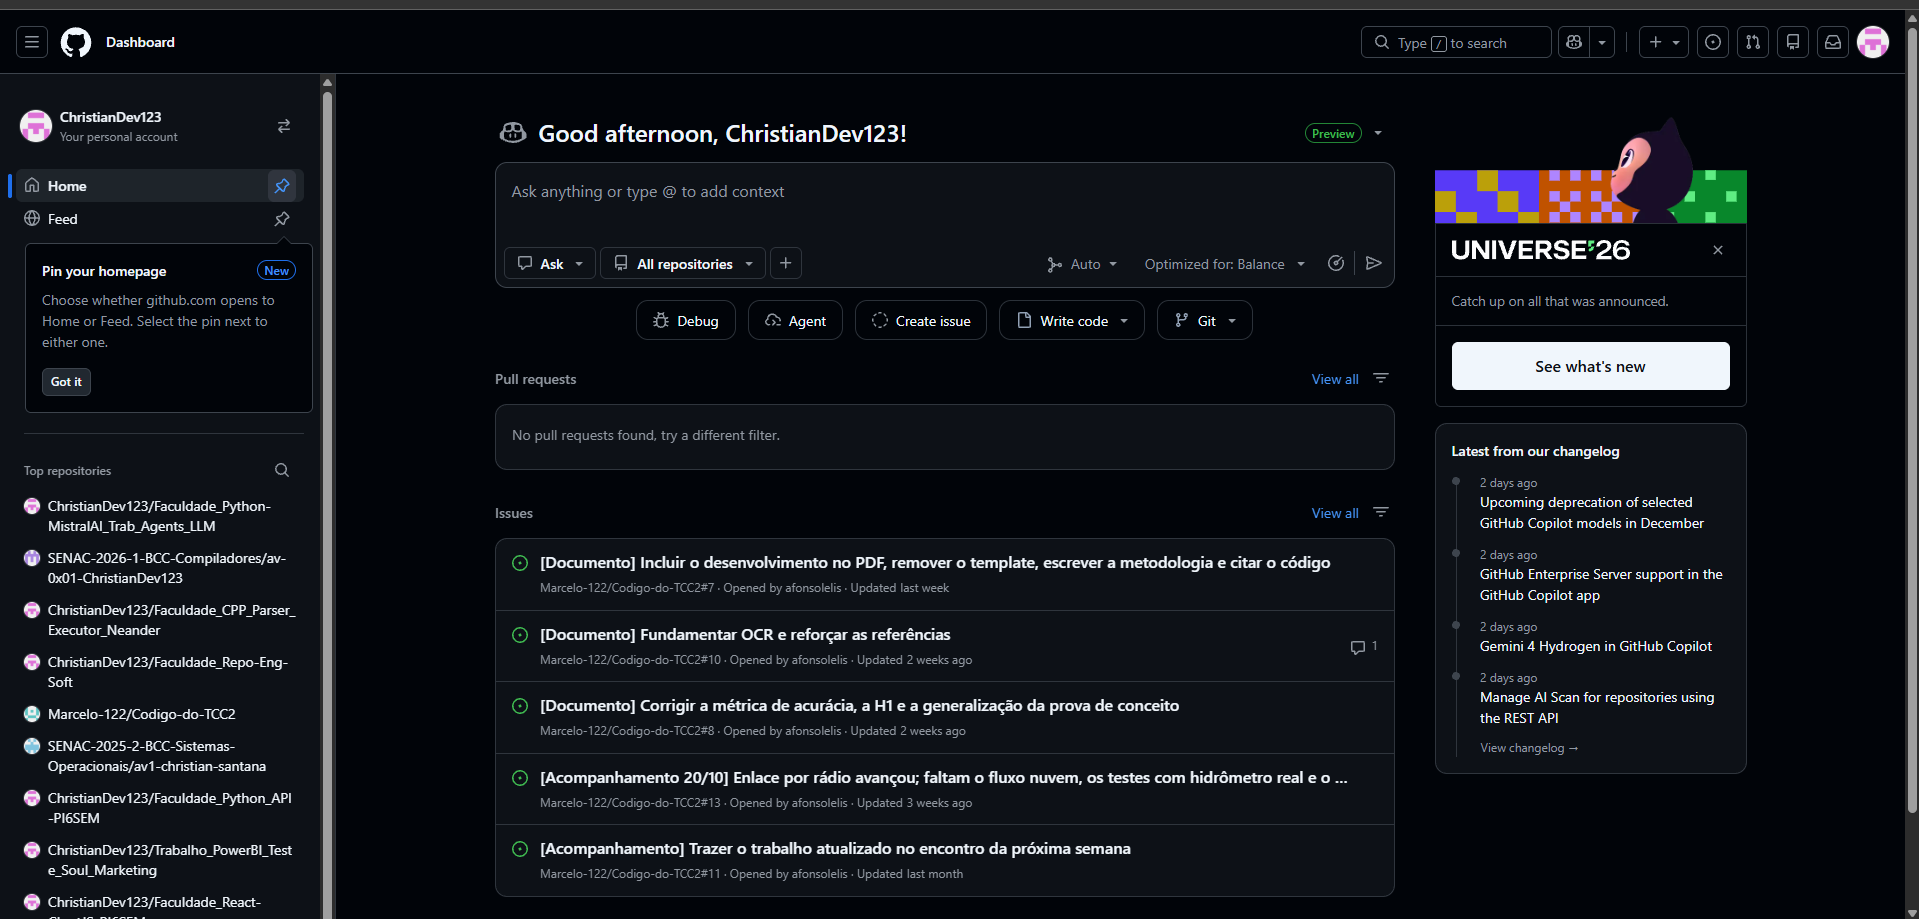
\includegraphics[width=0.8\textwidth]{sections/imagens/Github_Main_Page.png}
    \legend{Fonte: Captura de tela feita pelos autores (2026).}
\end{figure}

\subsubsection{Ferramentas para tratamento de imagens}
Durante a fase de pré-processamento dos dados utilizados no treinamento dos modelos de \gls{ocr} implementados, 
a utilização de determinadas ferramentas foi de extrema importância para o sucesso dessa etapa, destacando-se:

\begin{itemize}
	\item \textbf{NumPy}: Criada em 2005 por Travis Oliphant, é uma biblioteca focada em cálculos matriciais e algébricos.
	\item \textbf{OpenCV}: Lançada publicamente em 2000 e inicialmente desenvolvida pela Intel, é uma biblioteca voltada para o processamento de imagens e visão computacional.
	\item \textbf{h5py}: Criada em 2008 por Andrew Collette, é uma ferramenta voltada para gerenciar arquivos \texttt{.hdf5}, utilizados para armazenar de forma estruturada grandes volumes de dados vetoriais.
	\item \textbf{Pillow}: Em sua versão moderna, implementada em 2010 por Alex Clark e colaboradores, é uma biblioteca específica para manipulação e processamento de imagens.
	\item \textbf{Matplotlib}: Criada em 2003 por John D. Hunter, é uma das bibliotecas mais difundidas para a elaboração de gráficos e visualização de dados.
\end{itemize}

\subsubsection{Ferramentas para integração LoRa}
Durante o desenvolvimento das soluções comparadas,
foram utilizadas ferramentas baseadas em Python com o foco em administrar a comunicação, como é o caso do PySerial,
utilizado para gerenciar a comunicação serial entre o computador e as placas do transmissor e do receptor. Outro exemplo é o PyCryptodome, utilizado
para processar pacotes de rede trafegados via LoRaWAN, possibilitando a descriptografia com a chave AppSKey.